\subsection{Control de los invasores (Invaders)}
\label{invaders}

\begin{figure}[H]
	\centering
	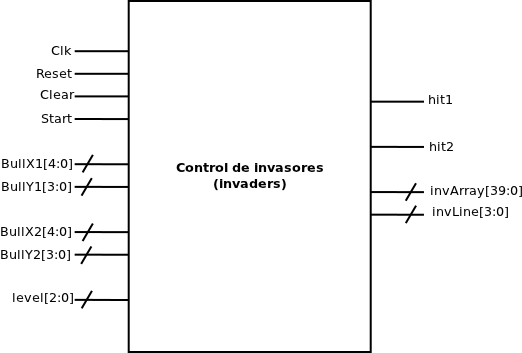
\includegraphics[width=0.4\textwidth]{invaders_block.png}
	\caption{Diagrama de bloques del Control de los invasores (Invaders) }\label{fig:invadersBlock}
\end{figure}

El bloque de control de los invasores se encarga tanto del movimiento de los invasores a lo largo de la pantalla, como de comprobar la posición del disparo y matar a los correspondientes marcianos. Para ello, además de las entradas de control típicas (Clk, Reset, Clear) posee 2 conjuntos de entradas que le proporcionan la posición y estado de cada una de las 2 balas del juego (una por cada jugador).

Para ello hemos definido una matriz constante que almacena la disposición inicial de los marcianos para cada uno de los 8 niveles implementados. Esta disposición se selecciona a través de la entrada ``level'', que indica el nivel actual.

Existen tres tipos de invasor, dependiendo del número de vidas que tengan (verde, 1 vida; amarillo, 2 vidas y blanco, 3 vidas) que se codifican usando 2 bits, siendo 00 un hueco sin marciano, 01 un marciano verde, 10 un marciano amarillo y 11 un marciano blanco, de 3 vidas. Estos marcianos se guardan en un vector de 40 elementos, 2 elementos por casilla de la pantalla en la que puede haber un marciano, que como se ha mencionado previamente, se selecciona dependiendo del nivel actual.

Este bloque también posee dos temporizadores que controlan la velocidad de avance de los invasores. Dependiendo del nivel se selecciona uno u otro, teniendo dos velocidades posibles (normal y rápida). Se seleccionó este diseño en lugar de un sólo temporizador con 8 velocidades (una por nivel) debido a que al haber aumentado la dificultad añadiendo marcianos más poderosos no tenía mucho sentido incrementarla aún más aumentando la velocidad en sólo 8 niveles, y había recursos suficientes en la FPGA como para poner dos teporizadores, cuyo diseño ya estaba realizado en prácticas anteriores, en lugar de uno nuevo con varias comprobaciones de cuenta.

La implementación en VHDL posee una señal ``start'', que sirve de señal de disparo, cambiando el estado de un biestable interno ``moving'' que indica al bloque que los marcianos han comenzado a moverse. Una vez en movimiento, cada pulso de reloj (en el que el temporizador lo permita), el vector de marcianos sufre un desplazamiento de 2 posiciones hacia la derecha. Si una de las 2 últimas posiciones del vector contiene un 1, es decir, si un marciano ha llegado al final de la línea, la posición en el eje Y se incrementa una unidad, y se invierte el sentido del desplazamiento. Este proceso se repite hasta que todos los marcianos hayan muerto, o hayan llegado a la última posición.

Por último se comprueba si el disparo coincide con la posición de alguno de los marcianos, y si es así, decrementa la vida del marciano en 1 unidad (un marciano blanco pasaría a ser amarillo, uno amarillo a ser verde, y uno verde moriría) y envía un pulso a través de la señal ``hit1'' o ``hit2'', dependiendo de qué jugador haya alcanzado al marciano.